\documentclass[11pt]{beamer}
\usepackage{graphicx,hyperref}
\usepackage{subfigure}
\usepackage[english]{babel}
\usepackage{times}
\usepackage[T1]{fontenc}
\usepackage{diagbox}
\usepackage[authordate]{biblatex-chicago}
\usepackage{setspace}
\usepackage{chngcntr}
\usepackage[table]{xcolor}
\usepackage{appendixnumberbeamer}
\usepackage{tikz}
\usepackage{csquotes}
\usepackage{longtable}
\usepackage{booktabs}
\usepackage{array}

\usetikzlibrary{arrows,positioning} 
\tikzset{
    %Define standard arrow tip
    >=stealth',
    %Define style for boxes
    punkt/.style={
           rectangle,
           rounded corners,
           draw=black, very thick,
           text width=6.5em,
           minimum height=2em,
           text centered},
    % Define arrow style
    pil/.style={
           ->,
           thick,
           shorten <=2pt,
           shorten >=2pt,}
}
\usepackage{hyperref}
\addbibresource{bib/PoliceResidency.bib}


\usetheme{Madrid}
\definecolor{EmoryBlue}{RGB}{1,33,105}
\usecolortheme[named=EmoryBlue]{structure}




    \title[Staggered Difference-in-Differences]{Staggered Difference-in-Differences}
    \author[Eric Dobbie]{Eric Dobbie}
    \institute[Emory]{Emory University\\Department of Political Science} 
    \date{\today}  
    \logo{
\includegraphics[width=1.19cm,height=0.4cm]{slidefigures/School.png}}

\begin{document}
%%%%%%%%%%%%%%%%%%%%%%%%%%%%%%%%%%%%%%%%%%%%%%%%%%%%%%%%%%%%%%%%%%%%%%%%%%%%%%%%%%%%%%
\begin{frame}\titlepage
\end{frame}


\begin{frame}{Staggered Treatment DiD}
    \begin{itemize}
        \item Common applied DiD settings are complicated, with treatments being applied at different time periods for different geographic units.
        \item These settings are especially common in policy evaluation settings, where policy is not adopted uniformly across different jurisdictions.
        \item Typical applied work used TWFE estimators in these applications. \textcite{chiu2026causal} find that about 60 out of 100 papers with staggered treatments use TWFE.
    \end{itemize}
\end{frame}

\begin{frame}{Goodman-Bacon Bias}
    \begin{itemize}
        \item However, TWFE has a problem. \textcite{goodman2021difference} showed that using TWFE leads to unintuitive comparisons, where the treatment group in a previous period serves as the control group for units treated in the current period.
        \item These comparisons bias the estimate of the ATT when using TWFE models
    \end{itemize}
\end{frame}

\begin{frame}{Goodman-Bacon Decomposition}
    \textcite{goodman2021difference} decomposes the TWFE model into all possible 2x2 DiD comparisons.

    \begin{figure}
        \centering
        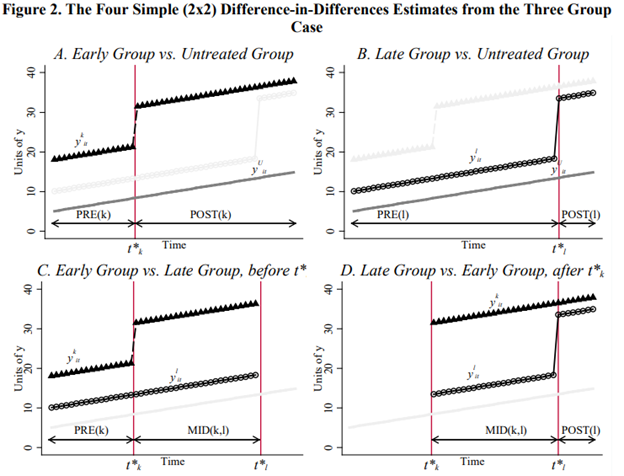
\includegraphics[width=0.7\linewidth]{slidefigures/comparisons.png}
        \label{fig:GB_Decomp}
    \end{figure}
\end{frame}

\begin{frame}{Goodman-Bacon Decomposition}
    There are two (related) problems that arise from this:

    \begin{enumerate}
        \item Some of these comparisons (namely Panel D) are unintuitive, strange comparisons
        \item When the late-vs-early comparisons are included, the already-treated cohort serves as the control, so changes in its treatment effect are subtracted. Those treatment effects enter the TWFE estimate with negative weight, biasing it whenever effects change over time.
    \end{enumerate}

     Because of these problems, TWFE estimators are generally not advisable in staggered treatment settings
\end{frame}


\section{Reweighting Estimators}

\begin{frame}{The Solution: Restrict Focus to Clean Comparisons}
    There is a class of modern estimators that works by restricting the analysis to clean comparisons of treated groups with not-yet-treated or never-treated control groups.

    \vspace{2.5mm}

   We will focus on a subset of these modern estimators. These estimators compute sub-experiment ATTs and aggregate them together, creating estimates that are a convex combination of each treatment cohort's effect (\cite{callaway2021difference, sun2021estimating, baker2026difference}). 

   \footnotesize 
   \vspace{5mm}
   
   Imputation estimators \parencite{borusyak2024revisiting} also estimate clean comparisons and aggregate. The difference is that they impute $Y(0)$ from a TWFE model fit on untreated observations, so every pre-period serves as the baseline rather than just $g-1$.
\end{frame}

\begin{frame}{Modern Estimators are Popular}
    These estimators are used a lot.
    \begin{itemize}
        \item \textcite{callaway2021difference} has been cited 15k times.
        \item \textcite{sun2021estimating} has been cited 10k times.
        \item \textcite{cengiz2019effect} and \textcite{wing2024stacked} have been cited 4k and 500 times respectively.
    \end{itemize}
\end{frame}


\begin{frame}{How do reweighting estimators work?}
    For a setting with $n$ treatment cohorts and $m$ time periods:
    
    \vspace{2.5mm}

    \begin{table}[]
\centering
\begin{tabular}{c|ccccc}
      \diagbox{g}{j}   & 1              & 2              & ...      & m-1              & m              \\ \hline
1        & $\tau_{1,1}$   & $\tau_{1,2}$   & ...      & $\tau_{1,m-1}$   & $\tau_{1,m}$   \\
2        & 0   & $\tau_{2,2}$   & ...      & $\tau_{2,m-1}$   & $\tau_{2,m}$   \\
$\vdots$ & $\vdots$       & $\vdots$       & $\vdots$ & $\vdots$         & $\vdots$       \\
n-1      & 0 & 0 & ...      & $\tau_{n-1,m-1}$ & $\tau_{n-1,m}$ \\
n        & 0  & 0   & ...      & $\tau_{n,m-1}$   & $\tau_{n,m}$  
\end{tabular}
\end{table}

    With treatment in period $k_g$, let $g \in [1,n]$ index treatment cohorts and $j \in [1,m]$ index time period, where $j \in [1,k_g)$ represent pre-treatment periods for each cohort and $j \in [k_g,m]$ represent treated periods. $\tau_{g,j}$ is the average treatment effect among the units of cohort $g$ in time $j$.

 

\end{frame}

\begin{frame}{Aggregating to the ATT}    
    \textcite{callaway2021difference} propose that researchers should use these as a target estimand and directly report these $\tau_{g,j}$ values. 

    \vspace{2.5mm}
    
    However, in settings where $g$ and/or $j$ are large, the number of $\tau_{g,j}$ values will be too large to take away substantive conclusions. 
    
\vspace{2.5mm}
    
    Therefore, many applied researchers look to aggregate these cohort by period effects into a more familiar aggregate ATT.
\end{frame}


\begin{frame}{Reasonable Aggregation Schemes}
    In order to aggregate these $\tau_{g,j}$ estimates, one can imagine several possible approaches:

    \begin{itemize}
        \item Aggregating over cohorts to generate event study or calendar estimates with period specific effects
        \item Aggregating over periods to generate cohort specific effects
        \item Aggregating over both periods and cohorts to generate a single ATT
    \end{itemize}
\end{frame}


\begin{frame}{Event Study Aggregation}
    For event study aggregation, the target is to reduce from $\tau_{g,j}$ to period specific effects, $\theta_{es}(e)$, where $e$ represents the number of periods since treatment for each cohort $g$. Formally, $e = j - k_g$. The event study estimate is given by:
    \begin{equation}
        \theta_{es}(e) = \sum_g w_{g,e} \tau_{g,k_g+e}
    \end{equation}

    Note that $e$ is cohort specific, such that $e = 1$ can be in different time periods $j$ for each cohort. 
\end{frame}

\begin{frame}{Event Study Aggregation}

    Consider an example with 5 time periods and 4 treatment cohorts, treated in periods 2 to 5 sequentially, such that cohort 1 is treated in period 2, cohort 2 is treated in period 3, and so on.

    \vspace{2.5mm}
    To aggregate to $\theta_{es}(0)$, the blue cells are added together using a weighted average, $\theta_{es}(1)$ is a weighted average of green cells, $\theta_{es}(2)$ is a weighted average of the purple cells, and $\theta_{es}(3) = \tau_{1,5}$, the orange cell, by construction:

    \begin{table}[]
\centering
\begin{tabular}{c|ccccc}
      \diagbox{g}{j}   & 1              & 2              & 3      & 4             & 5              \\ \hline
1        & 0   &\cellcolor{blue!30} $\tau_{1,2}$   & \cellcolor{green!30}$\tau_{1,3}$    & \cellcolor{purple!30}$\tau_{1,4}$   &\cellcolor{orange!30} $\tau_{1,5}$   \\
2        & 0   & 0  & \cellcolor{blue!30}$\tau_{2,3}$      & \cellcolor{green!30}$\tau_{2,4}$   & \cellcolor{purple!30}$\tau_{2,5}$   \\
3      & 0 & 0 &  0     & \cellcolor{blue!30}$\tau_{3,4}$ & \cellcolor{green!30}$\tau_{3,5}$ \\
4        & 0  & 0   & 0     & 0   & \cellcolor{blue!30}$\tau_{4,5}$  
\end{tabular}
\end{table}
\end{frame}


\begin{frame}{Calendar Effects}
    Another approach uses a calendar specific aggregation. Instead of normalizing to event time, one might be interested in the treatment effect at different points in time, so we aggregate over treatment cohorts within period $j$, for each cohort $g$ such that $j \geq k_g$.
    \begin{equation}
        \theta_c(j) = \sum_{g;j \geq k_g} w_{g,j} \tau_{g,j}
    \end{equation}
\end{frame}

\begin{frame}{Calendar Effects}
    Carrying forward the previous example,  $\theta_{c}(2) = \tau_{1,2}$, the blue cell, $\theta_{c}(3)$ is a weighted average of green cells, $\theta_{c}(4)$ is a weighted average of the purple cells, and $\theta_{c}(5)$ is a weighted average of the orange cells.

    \begin{table}[]
\centering
\begin{tabular}{c|ccccc}
      \diagbox{g}{j}   & 1              & 2              & 3      & 4             & 5              \\ \hline
1        & 0   &\cellcolor{blue!30} $\tau_{1,2}$   & \cellcolor{green!30}$\tau_{1,3}$    & \cellcolor{purple!30}$\tau_{1,4}$   &\cellcolor{orange!30} $\tau_{1,5}$   \\
2        & 0   & 0   & \cellcolor{green!30}$\tau_{2,3}$      & \cellcolor{purple!30}$\tau_{2,4}$   & \cellcolor{orange!30}$\tau_{2,5}$   \\
3      & 0 & 0 &  0     & \cellcolor{purple!30}$\tau_{3,4}$ & \cellcolor{orange!30}$\tau_{3,5}$ \\
4        &0  & 0   & 0     & 0   & \cellcolor{orange!30}$\tau_{4,5}$  
\end{tabular}
\end{table}
\end{frame}

\begin{frame}{Cohort Specific Effects}
    One could similarly imagine being interested in estimating the effects of a policy on each treatment cohort. For this, one would want to aggregate across time periods. 

    \begin{equation}
        \alpha_g = \sum_{j \geq k_g} w_{g,j} \tau_{g,j}
    \end{equation}
\end{frame}

\begin{frame}{Cohort Specific Effects}
    Returning to the example, to find cohort effects we aggregate over time within cohorts, so $\alpha_1$ is a weighted average of the blue cells, $\alpha_2$ is a weighted average of the green cells, $\alpha_3$ is a weighted average of the purple cells, and $\alpha_4 = \tau_{4,5}$, the orange cell.
    \begin{table}[]
\centering
\begin{tabular}{c|ccccc}
      \diagbox{g}{j}   & 1              & 2              & 3      & 4             & 5              \\ \hline
1        & 0   &\cellcolor{blue!30} $\tau_{1,2}$   & \cellcolor{blue!30}$\tau_{1,3}$    & \cellcolor{blue!30}$\tau_{1,4}$   &\cellcolor{blue!30} $\tau_{1,5}$   \\
2        & 0  & 0   & \cellcolor{green!30}$\tau_{2,3}$      & \cellcolor{green!30}$\tau_{2,4}$   & \cellcolor{green!30}$\tau_{2,5}$   \\
3      & 0 & 0 &  0     & \cellcolor{purple!30}$\tau_{3,4}$ & \cellcolor{purple!30}$\tau_{3,5}$ \\
4        & 0   & 0   & 0     & 0   & \cellcolor{orange!30}$\tau_{4,5}$  
\end{tabular}
\end{table}
\end{frame}

\begin{frame}{Single ATT Aggregation}
    The ATT for each of these reweighting estimators follows this general form:

    \begin{equation}\label{eq:delta}
        \delta = \sum_{g,\, j \geq k_g} w_{g,j} \tau_{g,j}
    \end{equation}

    Where $w_{g,j} \geq 0$ and $\sum_{g,j} w_{g,j} = 1$
\end{frame}

\begin{frame}{Single ATT Aggregation}
    To obtain a single ATT, all treated cells are combined using a weighted average to estimate $\delta$

    \begin{table}[]
\centering
\begin{tabular}{c|ccccc}
      \diagbox{g}{j}   & 1              & 2              & 3      & 4             & 5              \\ \hline
1        & 0  &\cellcolor{blue!30} $\tau_{1,2}$   & \cellcolor{blue!30}$\tau_{1,3}$    & \cellcolor{blue!30}$\tau_{1,4}$   &\cellcolor{blue!30} $\tau_{1,5}$   \\
2        & 0   & 0   & \cellcolor{blue!30}$\tau_{2,3}$      & \cellcolor{blue!30}$\tau_{2,4}$   & \cellcolor{blue!30}$\tau_{2,5}$   \\
3      & 0 & 0 &  0    & \cellcolor{blue!30}$\tau_{3,4}$ & \cellcolor{blue!30}$\tau_{3,5}$ \\
4        & 0   & 0   & 0     & 0   & \cellcolor{blue!30}$\tau_{4,5}$  
\end{tabular}
\end{table}
\end{frame}




\section{Stacked Regression}

\begin{frame}{Stacked Regression: Process}

In order to run a stacked regression (\cite{cengiz2019effect}):

\begin{enumerate}
    \item Select a window around treatment for the selection of clean controls, with equal number of periods before and after treatment.
    \item Identify clean controls based on selected control group (not-yet-treated or never-treated)
    \item Generate the ``stack'' with all units treated in time $t$ with all clean controls in the window selected.
\end{enumerate}

Once each stack has been formed, they are row binded together to form a full stacked dataset.
    
\end{frame}

\begin{frame}[label=stacked_est]{Stacked Regression: Estimation}
    The standard stacked regression setup then uses a two-way fixed effect estimator:

    \begin{equation}
        Y_{i,t} = \alpha_{i,s} + \gamma_{t,s} + \delta D_{i,t,s} + \epsilon
    \end{equation}

    where: 
    
    \begin{itemize}
        \item $\alpha_{i,s}$ is a unit by stack fixed effect
        \item $\gamma_{t,s}$ is a year by stack fixed effect
        \item $\delta$ is the ATT estimate.
    \end{itemize}

    \vfill
    \hfill\hyperlink{stack_decomp}{\beamergotobutton{Weight decomposition}}
\end{frame}

\newcolumntype{L}[1]{>{\raggedright\arraybackslash}p{#1}}

\section{Package Defaults}

\begin{frame}{Every Estimator Requires Choices}
Every estimator on the previous slides requires five choices:
\begin{enumerate}
  \item \textbf{Control group}: never-treated or not-yet-treated
  \item \textbf{Base period}: $g-1$, $t-1$, or an average of pre-periods
  \item \textbf{Estimating $\hat\tau_{g,t}$}: covariates and nuisance models
  \item \textbf{Aggregation weights}: how the $\tau_{g,t}$ become one number
  \item \textbf{Inference}: clustering, bootstrap, pointwise vs.\ uniform bands
\end{enumerate}
\vspace{0.5em}
If you do not make these choices, the package makes them for you.
Defaults differ across packages and across versions of the same packages, so think of these as a snapshot rather than a fixed thing.

\end{frame}

% ------------------------------------------------------------
\begin{frame}[fragile]{Callaway \& Sant'Anna: \texttt{did::att\_gt()}}
\scriptsize
\setlength{\tabcolsep}{3pt}
\begin{tabular}{L{2.9cm} L{2.5cm} L{6cm}}
\toprule
Argument & Default & What it does \\
\midrule
\verb|control_group| & \verb|"nevertreated"| & Only never-treated units as controls. \verb|"notyettreated"| adds later cohorts before they are treated. \\
\verb|base_period| & \verb|"varying"| & Post-treatment: $g-1$. Pre-treatment: $t-1$ (see the base-period slide). \\
\verb|anticipation| & \verb|0| & Base period is $g-1$; set $\delta>0$ to use $g-1-\delta$. \\
\verb|xformla| & \verb|NULL| & Unconditional DiD. With covariates (balanced panel), $X$ comes from the earlier period of each $2\times2$. \\
\verb|est_method| & \verb|"dr"| & \verb|DRDID::drdid_panel|: logit p-score (MLE) + OLS outcome model on controls. Only matters with covariates. \\
\verb|allow_unbalanced_|\newline\verb|  panel| & \verb|FALSE| & Units missing any period are silently dropped. \\
\verb|gname| coding & \verb|0| = never & Units treated in the first period are dropped. \\
\verb|bstrap|, \verb|cband| & \verb|TRUE|, \verb|TRUE| & Multiplier bootstrap (1000 draws), clustered on \verb|idname|, uniform bands. Set a seed. \\
\bottomrule
\end{tabular}

\vspace{0.6em}
\footnotesize
Note: the standalone \verb|DRDID::drdid()| has different defaults! Same authors, different default implementation.
\end{frame}

% ------------------------------------------------------------
\begin{frame}[fragile]{\texttt{did::aggte()} Defaults to \texttt{"group"}}
\footnotesize
The headline ``overall ATT'' depends on \verb|type|. With $p_g$ the share of units in cohort $g$:

\vspace{0.4em}
\setlength{\tabcolsep}{3pt}
\begin{tabular}{L{1.9cm} L{4cm} L{3cm}}
\toprule
\verb|type| & Overall ATT & Implied weight on cohort $g$ \\
\midrule
\verb|"group"| \textbf{(default)} & $\sum_g p_g\,\theta(g)$ & $\propto n_g$ \\
\verb|"simple"| & $\sum_{t\ge g} p_g\,\tau_{g,t} \big/ \sum_{t\ge g} p_g$ & $\propto n_g \times$ (\# post periods) \\
\verb|"dynamic"| & Simple average of $\theta_e(e)$ & Varies with $e$ \\
\verb|"calendar"| & Unweighted mean of $\theta_c(t)$ & Varies with $t$ \\
\bottomrule
\end{tabular}
\\[0.2em]

\vspace{0.6em}

These are four different estimands, not four estimates of one.
\end{frame}

% ------------------------------------------------------------
\begin{frame}{Varying vs.\ Universal Base Period}
With \texttt{base\_period = "varying"} (the default), one event-study plot shows two different objects:
\begin{itemize}
  \item \textbf{Post-treatment} ($t \ge g$): long differences, $t$ vs.\ $g-1$
  \item \textbf{Pre-treatment} ($t < g$): short differences, $t$ vs.\ $t-1$
\end{itemize}

\vspace{0.3em}
Consequences:
\begin{itemize}
  \item Pre-period coefficients are period-to-period changes, not cumulative deviations
        from $g-1$, so they are not comparable to post-period coefficients
  \item A linear differential trend of slope $s$ gives pre-period coefficients $\approx s$
        but post-period coefficients $\approx s(e+1)$: it looks like a break at $e=0$
  \item There is no omitted $e=-1$ reference point
\end{itemize}

\vspace{0.3em}
\texttt{base\_period = "universal"} compares every period to $g-1$, like a conventional
event study. Post-treatment $\hat\tau_{g,t}$ are unchanged.

\vspace{0.2em}
\scriptsize See \textcite{roth2026interpreting}
\end{frame}

% ------------------------------------------------------------
\begin{frame}[fragile]{Sun \& Abraham: \texttt{fixest::sunab()}}
\scriptsize
\setlength{\tabcolsep}{3pt}
\begin{tabular}{L{2.2cm} L{2.4cm} L{6.8cm}}
\toprule
Setting & Default & What it does \\
\midrule
\verb|ref.c| & \verb|NULL| & Never-treated cohorts are the controls; always-treated are dropped. \\
\verb|ref.p| & \verb|-1| & Universal base period, unlike CS's default. \\
\verb|summary(est)| & by $e$ & $\hat\delta_{g,e}$ averaged with weights $\propto$ \# observations in each cohort $\times$ $e$ cell (cohort shares). \\
\verb|agg = "ATT"| & --- & All $e\ge 0$ cells, observation-count weights $\propto n_g\times$(\# post periods). This is CS \verb|"simple"|. \\
Covariates & --- & Enter linearly with one common slope, not cohort-specific. \\
\verb|vcov| & \verb|"iid"| & Since fixest 0.13.0: \textbf{not clustered}, even with unit FE. Before 0.13.0: clustered by the first FE. \\
\verb|fixef.rm| & \verb|"perfect_fit"| & Since 0.13.0: singletons are removed. Point estimates unchanged; SEs can change. \\
\bottomrule
\end{tabular}

\vspace{0.6em}
\footnotesize
The package returns different standard errors depending on the installed version. Always pass \verb|cluster = ~id|.
\end{frame}

\begin{frame}{Stacked Regression}
    There is no standard R package for stacked regression. You would need to build the stacked dataset yourself and estimate the interactive model.

    \footnotesize
    \vspace{5mm}

    We don't recommend stacked regression anyways
\end{frame}


\section{End}



\begin{frame}{Questions?}
    
\end{frame}

\appendix

\begin{frame}[label=appendix]{Appendix Slides}
    \begin{itemize}
        \item \hyperlink{est_cs}{\beamergotobutton{Estimation of $\hat\tau_{g,t}$: Callaway \& Sant'Anna}}
        \item \hyperlink{est_sa}{\beamergotobutton{Estimation of $\hat\tau_{g,t}$: Sun \& Abraham}}
        \item \hyperlink{stack_decomp}{\beamergotobutton{Stacked regression weight decomposition}}
    \end{itemize}
\end{frame}


\section{Estimation}

\begin{frame}[label=est_cs]{Estimation of $\hat{\tau}_{g,t}$}
    Each of these three estimators uses a distinct approach to estimation of $\hat{\tau}_{g,t}$.

    \vspace{2mm}

    First, \cite{callaway2021difference} uses the following procedure:
    \begin{enumerate}
        \item Restrict the data to a subexperiment where we keep only units in
              cohort $g$ and the selected control group (never-treated or
              not-yet-treated), and periods $s = \{g-1,\, t\}$.
        \item Estimate propensity scores on that subsample $\mathcal{S}_{g,t}$:
    \end{enumerate}

    \vspace{-2mm}
    {\small
    \begin{align*}
      \hat\beta_{g,t}
        &= \arg\max_{\beta} \sum_{k \in \mathcal{S}_{g,t}}
           \Big[\, G_{g,k}\log \Lambda(X_k'\beta) \\[-0.5mm]
        &\hspace{26mm}
           + (1 - G_{g,k}) \log\big(1 - \Lambda(X_k'\beta)\big) \Big] \\[1mm]
      \hat\pi_{g,t}(X_k)
        &= \Lambda(X_k'\hat\beta_{g,t})
           \;\approx\; \Pr\big(G_{g,k} = 1 \mid X_k,\ G_{g,k} + C_k = 1\big)
    \end{align*}
    }
\end{frame}

\begin{frame}{Estimation of $\hat{\tau}_{g,t}$}
    \begin{enumerate}
        \item[3.] Fit an outcome model on control units only:
    \end{enumerate}

    \vspace{-2mm}
    {\small
    \begin{align*}
      \hat\gamma_{g,t}
        &= \arg\min_{\gamma} \sum_{k \in \mathcal{S}_{g,t}}
           C_k \Big( \Delta Y_k^{(g,t)} - X_k'\gamma \Big)^{2} \\[1mm]
      \hat\mu^{C}_{g,t}(X_k) &= X_k'\hat\gamma_{g,t}
    \end{align*}
    }

    \vspace{1mm}
    \begin{enumerate}
        \item[4.] Estimate the sub-experiment DiD with a doubly robust estimator.
              Writing $\hat o_k = \hat\pi_{g,t}(X_k) / \big(1 - \hat\pi_{g,t}(X_k)\big)$
              for the odds weight,
    \end{enumerate}

    \vspace{-2mm}
    {\small
    \begin{equation*}
      \widehat{\text{ATT}}^{\,dr}(g,t)
      = \frac{1}{n} \sum_{k \in \mathcal{S}_{g,t}}
        \left( \frac{G_{g,k}}{\widehat{\mathbb{E}}[G_g]}
             - \frac{\hat o_k \, C_k}{\widehat{\mathbb{E}}[\hat o \, C]} \right)
        \Big( \Delta Y_k^{(g,t)} - \hat\mu^{C}_{g,t}(X_k) \Big)
    \end{equation*}
    }

    \vfill
    \hfill\hyperlink{selecting}{\beamerreturnbutton{Back}}
    \hyperlink{appendix}{\beamerreturnbutton{Appendix}}
\end{frame}

\begin{frame}[label=est_sa]{Estimation of $\hat{\tau}$}

\cite{sun2021estimating} have a distinct approach, estimating one interactive model on the full sample:

\begin{align*}
  Y_{it}
  \;&=\;
  \alpha_i + \lambda_t
  + \sum_{g \notin C} \; \sum_{\ell \neq -1}
    \delta_{g,\ell} \Big( \ind{G_i = g} \cdot \ind{t - g = \ell} \Big)
  + \varepsilon_{it}, \\
  &\qquad
  \widehat{\CATT}_{g,\ell} \;=\; \hat\delta_{g,\ell}.
\end{align*}

    \vfill
    \hfill\hyperlink{selecting}{\beamerreturnbutton{Back}}
    \hyperlink{appendix}{\beamerreturnbutton{Appendix}}
\end{frame}


\section{Stacked Regression Decomposition}

\begin{frame}[label=stack_decomp]{Stacked Regression Weight Decomposition: Setup}
    In the pooled stacked regression, outcomes can be expressed as:
    \[
        y_{its} = \gamma_{is} + \delta_{ts} + \beta D_{its} + \epsilon_{its}
    \]
    where $\gamma_{is}$ is a unit-by-stack fixed effect and $\delta_{ts}$ is a
    time-by-stack fixed effect.

    \vspace{3mm}

    We start by partialling out the fixed effects from the treatment:
    \[
        D_{its} = a_{is} + g_{ts} + v_{its}
    \]
    Where $a_{is}$ and $g_{ts}$ are the fitted effects from projecting $D$ onto
    the unit-by-stack and time-by-stack dummies. By FWL, $\hat{\beta}$ is
    recovered from the regression of $y$ on $\hat{v}$:
    \[
        \hat{\beta} =
        \frac{\sum_s \sum_{i,t \in s} \hat{v}_{its} y_{its}}
             {\sum_s \sum_{i,t \in s} \hat{v}_{its}^2}
    \]
\end{frame}

\begin{frame}{Lemma 1 (Stack Partitions)}
    \begin{block}{Lemma 1}
        When the unit and time fixed effects are stack-interacted, the full
        system of $\sum_s (N_s + T_s)$ normal equations partitions into $S$
        independent subsystems, the $s$-th being the two-way dummy regression of
        $D$ on stack $s$'s rows alone.
    \end{block}

    \vspace{3mm}

    The pooled regression can be decomposed to individual stack regressions.
    First, we partial out the fixed effects from treatment assignment and solve
    for the first order conditions:
    \[
        \min_{\{a_{is}\}\{g_{ts}\}}
        \sum_{s=1}^{S} \sum_{i \in I_s} \sum_{t \in T_s}
        \left[ D_{its} - a_{is} - g_{ts} \right]^2
    \]
    where $I_s$ is the set of units in stack $s$ and $T_s$ is the periods in
    stack $s$.
\end{frame}

\begin{frame}{Lemma 1: Why the Interaction Matters}
    Note that, for any unit that appears in multiple stacks, say $s$ and $s'$,
    as a clean control, $a_{is}$ and $a_{is'}$ are separate parameters that are
    not necessarily equal.

    \vspace{3mm}

    With a stack-interacted $a_{is}$ the FOC for the parameter involves only
    rows within the stack $s$. Otherwise, a single $a_i$ appears in the FOC of
    rows from every stack containing unit $i$ and the normal equations no longer
    partition.

    \vspace{5mm}

    \footnotesize
    This is why using $a_i$ without stack interacting is problematic for the purposes of the decomposition. The $a_i$ parameter enters across all stacks containing unit $i$, making the within stack estimation problem dependent on other stacks.
\end{frame}

\begin{frame}{Lemma 1: Solving the First Order Conditions}
    \[
        \frac{\partial}{\partial a_{is}}: \quad
        -2 \sum_{t \in T_s} \left[ D_{its} - a_{is} - g_{ts} \right] = 0
    \]
    Solving for $a$:
    \[
        a_{is} = \bar{D}_{i \cdot s} - \bar{g}_s,
        \qquad
        \bar{D}_{i \cdot s} = \frac{1}{T_s} \sum_{t \in T_s} D_{its},
        \qquad
        \bar{g}_s = \frac{1}{T_s} \sum_{t \in T_s} g_{ts}
    \]
    Using the same logic, the first order condition with respect to $g$ gives:
    \[
        g_{ts} = \bar{D}_{\cdot ts} - \bar{a}_s,
        \qquad
        \bar{D}_{\cdot ts} = \frac{1}{N_s} \sum_{i \in I_s} D_{its},
        \qquad
        \bar{a}_s = \frac{1}{N_s} \sum_{i \in I_s} a_{is}
    \]

    \vspace{3mm}

    Every parameter carries the stack index $s$, and every FOC ranges only over
    rows of that stack. No parameter is shared across stacks, so the system
    partitions as claimed. \hfill $\blacksquare$
\end{frame}

\begin{frame}{Corollary 1 (Two-Way Demeaning)}
    \begin{block}{Corollary 1}
        If a stack $s$ is balanced, the subsystem-$s$ residual is
        $\hat{v}_{its} = D_{its} - \bar{D}_{i \cdot s} - \bar{D}_{\cdot ts} + \bar{D}_{\cdot \cdot s}$.
    \end{block}

    Without loss of generality, normalizing $\bar{a}_s = 0$ such that
    $g_{ts} = \bar{D}_{\cdot ts}$ so $\bar{g}_s = \bar{D}_{\cdot \cdot s}$.
    Plugging back into $a_{is} = \bar{D}_{i \cdot s} - \bar{g}_s$:
    \[
        a_{is} = \bar{D}_{i \cdot s} - \bar{D}_{\cdot \cdot s}
    \]
    Which satisfies $\bar{a}_s = 0$ as, once we average over the units,
    $\bar{D}_{\cdot \cdot s} - \bar{D}_{\cdot \cdot s} = 0$.

    \vspace{3mm}

    Plugging back in to $\hat{D}_{its} = a_{is} + g_{ts}$:
    \[
        \hat{D}_{its} = \bar{D}_{i \cdot s} + \bar{D}_{\cdot ts} - \bar{D}_{\cdot \cdot s}
        \qquad \Longrightarrow \qquad
        \hat{v}_{its} = D_{its} - \bar{D}_{i \cdot s} - \bar{D}_{\cdot ts} + \bar{D}_{\cdot \cdot s}
    \]
\end{frame}

\begin{frame}{Corollary 1: Verifying the FOCs}
    Plugging in to the unit FOC:
    \[
        \sum_{t \in T_s} \hat{v}_{its}
        = T_s \bar{D}_{i \cdot s} - T_s \bar{D}_{i \cdot s}
          - T_s \bar{D}_{\cdot \cdot s} + T_s \bar{D}_{\cdot \cdot s} = 0
    \]
    and the time FOC:
    \[
        \sum_{i \in I_s} \hat{v}_{its}
        = N_s \bar{D}_{\cdot ts} - N_s \bar{D}_{\cdot \cdot s}
          - N_s \bar{D}_{\cdot ts} + N_s \bar{D}_{\cdot \cdot s} = 0
    \]

    \vspace{3mm}

    \textbf{Assumption: Balanced Panel.} Note that
    $\sum_{t \in T_s} \bar{D}_{\cdot ts} = T_s \bar{D}_{\cdot \cdot s}$ and
    $\sum_{i \in I_s} \bar{D}_{i \cdot s} = N_s \bar{D}_{\cdot \cdot s}$ hold if
    the stack is balanced such that every unit $I_s$ is observed in every period
    $T_s$. This assumption is only necessary for Corollary 1. It is not
    necessary for Lemma 1 or the remaining portions of the proof.
\end{frame}

\begin{frame}{Lemma 2 (Stack-Specific Coefficients)}
    \begin{block}{Lemma 2}
        In the saturated model, $\hat{\beta}_r$ is identical to the coefficient
        from regressing $y$ on $D$ using the data from stack $r$ alone, provided
        $\sum_{i,t \in r} \hat{v}_{itr}^2 > 0$.
    \end{block}

    Now, allow for each stack to have its own treatment coefficient:
    \[
        D^{(r)}_{its} = D_{its} \cdot \mathbf{1}\{s = r\}
    \]
    So $D^{(r)}$ equals the treatment indicator on stack-$r$ rows and zero
    elsewhere. The saturated model is:
    \[
        y_{its} = \alpha_{is} + \gamma_{ts}
        + \sum_{r=1}^{S} \beta_r D^{(r)}_{its} + \epsilon_{its}
    \]
    Each $\beta_r$ is the treatment coefficient for stack $r$. On a row in stack
    $s$, only the $r = s$ term is nonzero.
\end{frame}

\begin{frame}{Lemma 2: Partialling Out}
    For each stack's $\beta_r$, we can partial out the stack-by-unit and
    stack-by-time dummies from the treatment indicator, as before:
    \[
        \min_{\{a^{(r)}_{is}\}\{g^{(r)}_{ts}\}}
        \sum_{s=1}^{S} \sum_{i \in I_s} \sum_{t \in T_s}
        \left[ D^{(r)}_{its} - a^{(r)}_{is} - g^{(r)}_{ts} \right]^2
    \]
    This is the same minimization problem as in Lemma 1 with $D$ replaced by
    $D^{(r)}$. Applying Lemma 1, the problem separates into $S$ independent
    subsystems. For a subsystem $s \neq r$, all rows of the treatment indicator
    are equal to zero:
    \[
        \min_{\{a^{(r)}_{is}\}\{g^{(r)}_{ts}\}}
        \sum_{i \in I_s} \sum_{t \in T_s}
        \left[ 0 - a^{(r)}_{is} - g^{(r)}_{ts} \right]^2
    \]
    Which is minimized at $a^{(r)}_{is} = g^{(r)}_{ts} = 0$, meaning
    $\hat{v}^{(r)}_{its} = 0$ for all $i, t$ in any stack $s \neq r$.
\end{frame}

\begin{frame}{Lemma 2: Orthogonality and Collapse}
    Within subsystem $r$ itself, the problem collapses back to the single
    coefficient model solved before and
    $\hat{v}^{(r)}_{itr} = D_{itr} - \bar{D}_{i \cdot r} - \bar{D}_{\cdot tr} + \bar{D}_{\cdot \cdot r} = \hat{v}_{itr}$.

    \vspace{2mm}

    As a consequence, the residual regressors are mutually orthogonal such that
    for $r \neq r'$, the product $\hat{v}^{(r)}_{its} \hat{v}^{(r')}_{its} = 0$,
    as wherever the first term is nonzero, the second term is zero and vice
    versa, and $\sum_s \sum_{i,t \in s} \hat{v}^{(r)}_{its} \hat{v}^{(r')}_{its} = 0$.

    \vspace{2mm}

    Because partialled out regressors are uncorrelated with each other, the
    multivariate least squares solution collapses to the univariate solution
    applied separately:
    \[
        \hat{\beta}_r =
        \frac{\sum_s \sum_{i,t \in s} \hat{v}^{(r)}_{its} y_{its}}
             {\sum_s \sum_{i,t \in s} (\hat{v}^{(r)}_{its})^2}
        \qquad \Longrightarrow \qquad
        \hat{\beta}_r =
        \frac{\sum_{i,t \in r} \hat{v}_{itr} y_{itr}}
             {\sum_{i,t \in r} (\hat{v}_{itr})^2}
    \]
    All terms with $s \neq r$ are equal to zero and drop out. \hfill $\blacksquare$
\end{frame}

\begin{frame}{Lemma 2: The Regularity Condition}
    This solution requires
    \[
        \sum_{i,t \in r} (\hat{v}_{itr})^2 > 0
    \]
    or that the treatment retains variation after within-stack partialling out.

    \vspace{3mm}

    When this fails, coefficients within those stacks cannot be estimated. As
    such, $\hat{\beta}_r$ does not exist in these cases and they are excluded
    from the decomposition.

    \vspace{3mm}

    Hence, $\hat{\beta}_r$ is identical to the coefficient from the regression of
    $y$ on $D$ within stack $r$'s data.
\end{frame}

\begin{frame}{Proposition 1 (Weight Decomposition)}
    \begin{block}{Proposition 1}
        The pooled stacked coefficient is a weighted average of the
        stack-specific coefficients.
        \[
            \hat{\beta} = \sum_s w_s \hat{\beta}_s,
            \qquad
            w_s = \frac{V_s}{V},
            \quad
            V_s = \sum_{i,t \in s} \hat{v}_{its}^2,
            \quad
            V = \sum_{s=1}^{S} V_s
        \]
    \end{block}

    The weights are the share of total residualized treatment variation. Weights
    are non-negative and sum to one as $V_s$ is a sum of squares and
    $\sum_s w_s = \sum_s V_s / V = 1$. The weights are taken over stacks that
    satisfy the regularity condition.
\end{frame}

\begin{frame}{Proposition 1: Substitution}
    We can rewrite $\sum_{i,t \in r} \hat{v}_{itr} y_{itr}$ as:
    \[
        \sum_{i,t \in r} \hat{v}_{itr} y_{itr}
        = \hat{\beta}_r \sum_{i,t \in r} \hat{v}_{itr}^2
    \]
    Substituting into the pooled expression:
    \[
        \hat{\beta}
        = \frac{\sum_s \hat{\beta}_s \sum_{i,t \in s} \hat{v}_{its}^2}{V}
        = \frac{\sum_s \hat{\beta}_s V_s}{V}
        = \sum_s w_s \hat{\beta}_s
        \qquad \blacksquare
    \]

    \vspace{5mm}

    \footnotesize
    This property only holds under stack-interacted fixed effects, not as a
    general property of all stacked regressions. Wing, Freedman, and
    Hollingsworth (2024) state this convexity for a stacked fixed-effect
    specification under the additional condition that treatment share is constant
    across sub-experiments. It appears that this additional condition is
    unnecessary, as the within-stack FOC in Lemma 1 force the residualized
    treatment to have zero mean within each stack.

    \vfill
    \hfill\hyperlink{stacked_est}{\beamerreturnbutton{Back}}
    \hyperlink{appendix}{\beamerreturnbutton{Appendix}}
\end{frame}


\end{document}